\documentclass[11pt,Chicago]{uuthesis}

% SETUP
\usepackage{amssymb}
\usepackage{graphicx}
\usepackage{caption}
\usepackage{subcaption}
\usepackage{multicol}
\usepackage{adjustbox}
\usepackage{amsmath}
\usepackage[utf8]{inputenc}
\usepackage[usenames,dvipsnames,svgnames,table]{xcolor}
\usepackage{listings}
\lstset{
    language=C, % choose the language of the code
    basicstyle=\ttfamily,
    keywordstyle=\color{ForestGreen},
    identifierstyle=\color{Blue},
    numbers=none, % where to put the line-numbers
    numberstyle=\tiny, % the size of the fonts that are used for the
                       % line-numbers      
    showspaces=false, % show spaces adding particular underscores
    showstringspaces=false, % underline spaces within strings
    showtabs=false, % show tabs within strings adding particular underscores
    frame=single, % adds a frame around the code
    tabsize=2, % sets default tabsize to 2 spaces
    rulesepcolor=\color{gray},
    rulecolor=\color{black},
    captionpos=b, % sets the caption-position to bottom
    breaklines=false, % sets automatic line breaking
    breakatwhitespace=false, 
}

%Boogie stuff from Rustan Leino -
%https://github.com/hesam/SketchSharp/blob/master/Boogie/Util/latex/boogie.sty
\lstdefinelanguage{boogie}{
  morekeywords={type,finite,bool,int,ref,%
      bv0,bv1,bv2,bv3,bv4,bv5,bv6,bv7,bv8,bv9,%
      bv10,bv11,bv12,bv13,bv14,bv15,bv16,bv17,bv18,bv19,%
      bv20,bv21,bv22,bv23,bv24,bv25,bv26,bv27,bv28,bv29,%
      bv30,bv31,bv32,bv33,bv34,bv35,bv36,bv37,bv38,bv39,%
      bv40,bv41,bv42,bv43,bv44,bv45,bv46,bv47,bv48,bv49,%
      bv50,bv51,bv52,bv53,bv54,bv55,bv56,bv57,bv58,bv59,%
      bv60,bv61,bv62,bv63,bv64,% ...
      const,unique,complete,partition,
      axiom,
      function,returns,
      var,where,
      procedure,implementation,
      requires,modifies,ensures,free,
      % expressions
      false,true,null,old,then,
      % statements
      assert,assume,havoc,call,if,else,while,invariant,break,return,goto,
      },
  literate=%
    %{:}{$\colon$}1
    %{::}{$\bullet$}2
    %{:=}{$:$$=$}2
    %{!}{$\lnot$}1
    %{==}{$=$}1
    %{!=}{$\neq$}1
    %{&&}{$\land$}1
    %{||}{$\lor$}1
    %{<=}{$\le$}1
    %{=>}{$\ge$}1
    %{==>}{$\Longrightarrow$}3 
    %{<==>}{$\Longleftrightarrow$}4 
    %{forall}{$\forall$}1
    %{exists}{$\exists$}1
    %{lambda}{$\lambda$}1
    % the following isn't actually Boogie, but it gives the option to
    % produce nicer latex 
    {<<}{$\langle$}1
    {>>}{$\rangle$}1
    {\\alpha}{$\alpha$}1
    {\\beta}{$\beta$}1
    {\\gamma}{$\gamma$}1
    {\\delta}{$\delta$}1
    {\\epsilon}{$\epsilon$}1
    {\\zeta}{$\zeta$}1
    {\\eta}{$\eta$}1
    {\\theta}{$\theta$}1
    {\\iota}{$\iota$}1
    {\\kappa}{$\kappa$}1
    {\\lambda}{$\lambda$}1
    {\\mu}{$\mu$}1
    {\\nu}{$\nu$}1
    {\\xi}{$\xi$}1
    {\\pi}{$\pi$}1
    {\\rho}{$\rho$}1
    {\\sigma}{$\sigma$}1
    {\\tau}{$\tau$}1
    {\\upsilon}{$\upsilon$}1
    {\\phi}{$\phi$}1
    {\\chi}{$\chi$}1
    {\\psi}{$\psi$}1
    {\\omega}{$\omega$}1
    {\\Gamma}{$\Gamma$}1
    {\\Delta}{$\Delta$}1
    {\\Theta}{$\Theta$}1
    {\\Lambda}{$\Lambda$}1
    {\\Xi}{$\Xi$}1
    {\\Pi}{$\Pi$}1
    {\\Sigma}{$\Sigma$}1
    {\\Upsilon}{$\Upsilon$}1
    {\\Phi}{$\Phi$}1
    {\\Psi}{$\Psi$}1
    {\\Omega}{$\Omega$}1
    ,
  sensitive=true,  % case sensitive
  morecomment=[l]{//},
  morecomment=[s]{/*}{*/},
  morestring=[b]",
}


\fourlevels
\setcounter{tocdepth}{4}

% INFO
\title{Modeling Concurrency:\protect\\Extending SMACK to Support Pthreads}
%Supporting pthreads in SMACK verifier
%Pthreads extension for SMACK verifier
\author{Montgomery Carter}
\supervisor{Zvonimir Rakamarić}
\submitdate{May 2015}
\copyrightyear{2015}
\thesistype{thesis}


\usepackage{hyperref}
\hypersetup{
    colorlinks,
    citecolor=black,
    filecolor=black,
    linkcolor=black,
    urlcolor=black,
    bookmarksopen=true,
    bookmarksopenlevel=0
}
\usepackage{bookmark}

%%% Generate pdfbookmarks in lof & lot for all figures and tables
\usepackage{etoolbox}
\makeatletter
\pretocmd\endfigure{%
\addtocontents{lof}{\protect{%
    \bookmark[
    rellevel=1,
    keeplevel,
    dest=\@currentHref,
    ]{Figure \thefigure: \@currentlabelname}}}%
}{}{\errmessage{Patching \noexpand\endfigure failed}}

\pretocmd\endtable{%
\addtocontents{lot}{\protect{%
    \bookmark[
    rellevel=1,
    keeplevel,
    dest=\@currentHref,
    ]{Table \thefigure: \@currentlabelname}}}%
}{}{\errmessage{Patching \noexpand\endtable failed}}
\makeatother

% DOCUMENT
\begin{document}


% front matter
\frontmatterformat
\titlepage
%Add Root node to pdfbookmark, point it to toc
\bookmark[level=-1,dest=tocBM]{Contents}
\preface{thesis_abstract}{Abstract}
\clearpage
\hypertarget{tocBM}{}%
\addtocontents{toc}{\protect\sloppy}
\tableofcontents
\listoffigures
\listoftables
%With lot & lof bookmarks not expanded, switch to next depth to expand
%chapters node
\hypersetup{bookmarksopenlevel=1}
\preface{thesis_acknowledge}{Acknowledgments}

% body
\maintext
%Set chapters down a level for pdf bookmarks
\makeatletter
\renewcommand{\toclevel@chapter}{1}
\renewcommand{\toclevel@section}{2}
\renewcommand{\toclevel@subsection}{3}
\renewcommand{\toclevel@subsubsection}{4}
\renewcommand{\toclevel@paragraph}{5}
\renewcommand{\toclevel@subparagraph}{6}
\makeatother
\chapter{Introduction}\label{ch:introduction}

Verification of programs using formal methods has long been a
promising area whose practical adoption has gone unrealized.  Recent
advances in computing performance and verification algorithms have
made these well-understood formal verification techniques available
for real world applications.  As practical adoption of formal
verification becomes a reality, it has become necessary to create
tools that address the use cases where formal verification will
be most advantageous. 

One such use case is the verification of concurrent programs.  As
multi-core systems become more ubiquitous, the parallel programming
paradigm is increasingly relevant.  Parallel programming presents a
unique challenge for developers, as an extra dimension of complexity
is introduced.  Indeed, concurrent programs can suffer from a host of
issues that simply do not apply to the sequential programming
paradigm, such as race conditions and deadlocks.  As a result,
verification tools suited for real world usage should support
concurrency.

SMACK is a bounded software verification tool for C/C++ programs, and
is the result of a joint effort between the University of Utah, IMDEA
Software Institute, and Microsoft Research~\cite{smack}.  With a
growing user base and active support from both the academic and
industry communities, it is a good candidate for continued
development.  SMACK, however, currently lacks support for any form of
concurrency.  Requests from the SMACK user community have encouraged
the SMACK development team to add support for the pthread library as
its first supported concurrency paradigm.   As such, though pthreads
support is implemented in other formal verification tools, the
community benefits from extending SMACK with a model to support
abstract interpretation of C/C++ programs that utilize the pthreads
library.  

SMACK utilizes an intermediate verification language (IVL) called
Boogie, which separates the semantic modeling of input source programs
from the processes and algorithms involved in verifying modeled input
programs.  Rather than directly model checking libraries included by
input source programs, modeling the behavior of included libraries is
the preferred method for verifying input programs utilizing such
libraries.  This reduces both the computational and engineering
complexity required to verify input programs including such libraries,
as details such as the underlying hardware, operating system and error
handling are abstracted away in the models being checked.

It follows, then, that extending SMACK to support the verification of
input programs that include the pthread library requires designing a
model that express the behavior of the pthread library using the
modeling environment available in SMACK.  Designing such a model for
the pthread API requires investigating and understanding the
underlying constructs needed for expressing the behavior of concurrent
programming paradigms in general.  This leads to the thesis of this
paper:

\begin{quote}
\begin{center}
\textbf{Thesis Statement}
\end{center}
``The complex behavior of the pthread
API can be accurately modeled using the set of basic concurrency
modeling primitives available in the SMACK modeling environment,
allowing SMACK to accurately verify input programs utilizing the
pthread library.''
\end{quote}

In this paper, I demonstrate that SMACK can indeed be used to
accurately model the pthread library.  First, I discuss in further
detail the SMACK verification framework.  Having introduced SMACK, I
proceed to detail the process of developing a model which captures the
behavior of the pthread library function calls. Next, I describe the
actual implementation of support for pthreads in the SMACK toolchain,
allowing for the verification of concurrent programs.  Finally, I
highlight the empirical testing performed on the pthread extension to
SMACK which demonstrates the accuracy of the implementation. 

%%% Local Variables: 
%%% mode: latex
%%% TeX-master: "thesis"
%%% End: 

\chapter{Related Work}\label{thesis_relatedwork}
Related works
%%% Local Variables: 
%%% mode: latex
%%% TeX-master: t
%%% End: 

\chapter{SMACK Verification Framework}\label{ch:smackframework}
SMACK is part of a modular software verification framework which is
built on top of the Boogie intermediate verification language (IVL),
and aims to reduce the large engineering effort typically required for
implementing bounded software verification tools.  This chapter first
provides some background for SMACK's verification framework, then
introduces the SMACK toolchain, and finally, discusses the
environment presented by the framework for modeling input program
behavior.  

\section{Framework Background}
Developing a fully featured bounded software verification tool from
end-to-end can be a daunting task.  Bounded model checking requires
several steps.  First, the input source code must be parsed or
compiled.  The resulting abstract syntax tree (AST) must then be
semantically interpreted, and a model built of underlying program
semantics. Finally, the modeled program must be represented as a
satisfiability modulo theories (SMT) query and passed through an SMT
solver.  This imposes a large barrier to entry for prototyping a new
model checking algorithm, or building a verification tool for a new
source language using existing algorithms. 

The Boogie intermediate verification language (IVL) was designed by
Microsoft Research to alleviate the complexity of modeling new source
languages and implementing new model checking algorithms.  Boogie IVL
separates the task of modeling input program semantics from the task
of bounding and checking modeled programs.  This allows model checking
tools to take Boogie IVL files as input, rather than the input source
language.  Similarly, front-end tools can model the input program
semantics in Boogie IVL rather than being directly integrated with
the model checker.  By providing a layer of abstraction between the
tasks of modeling input source programs and the checking of modeled
programs, Boogie IVL enables the development of components in a
modular fashion.  The resulting components can be roughly separated
into two categories: front-end modeling tools, and
back-end solvers.

\subsection{Front End Modelers}\label{sec:frontends}
Due to its goal of creating an abstraction between program modeling
and model checking, Boogie IVL has been designed to be a very
low-level modeling language.  It contains support for little more than
a typing system, basic arithmetic expressions \& statements, control
flow \& procedure calls, and verification condition
specification~\cite{boogie}.  Any more complicated semantics of the
source language must be modeled using the basic set of primitives
available in Boogie IVL.

Though the low-level nature of Boogie IVL provides the flexibility to
support a large variety of models of computation and source languages,
it requires that models be created to define the semantics of
operations available within the source language and computational
model environments.  As an example, there is no concept of a heap
within Boogie.  Because of this, a memory model must be developed that
accurately models the behavior of the heap.  A rudimentary model of
memory could use a simple, large array of integers to represent the
heap, where each element represents a word of memory, and C pointers
are simply indices into this array.

The SMACK tool itself, which translates C/C++ code into Boogie IVL, is
one example of a front-end for this framework.  There are several
other front-ends, which provide support for mainstream programming
languages such as .NET and Java, in addition to verification and
prover languages like Dafny and Chalice.

\subsection {Back End Solvers}
The original back-end solver for Boogie IVL programs is a tool called
Boogie.  (To ease discussion, ``Boogie'' will hereafter refer to
Boogie IVL, while ``Boogie verifier'' will refer to the back end
solver.)  In addition to being a complete back-end verifier for Boogie
programs, it also provides an API for parsing Boogie IVL and 
interfacing with SMT solvers. As the goal of Boogie is to modularize
model checking verifiers, it should not be surprising that there are
several additional back-end solvers that perform verification of
Boogie programs, such as Corral and Duality.  

Corral is one of the more popular back-end solvers for Boogie
programs, and also happens to be an excellent example of how Boogie
has simplified the implementation of new model checking algorithms.
Corral leverages the Boogie verifier's API to parse Boogie code and
interface with SMT solvers~\cite{corral}.  However, Corral implements
model checking algorithms not available with the Boogie verifier, such
as the Lal/Reps sequentialization algorithm~\cite{LalReps}. Indeed,
Corral has put considerable effort toward providing support for
verification of concurrent programs.  As such, it was the ideal
candidate to use as a back-end verifier for the pthreads extension of
SMACK. 

However, although providing state of the art algorithms for checking
concurrent programs, Corral is similar to the Boogie IVL in that it
provides only low-level support for modeling concurrency.  The Corral
program verifier provides an extension to Boogie IVL that includes a
very basic set of primitives for modeling concurrent programs.  The
behavior prescribed in the pthread specification~\cite{pthreads} is
much more complex than these low-level concurrency primitives
recognized by Corral.  As a result, to provide support for the more
complex pthread API within SMACK, it is necessary to build a model
capturing the behavior of the pthread API, using the primitives
provided by Corral. 


\section{SMACK Toolchain}\label{sec:smacktoolchain}
As mentioned in Section~\ref{sec:frontends}, the SMACK tool itself is
a front-end for the verification framework centered around Boogie.
However, at its core, it is essentially a compiler that takes C/C++
programs and translates them into Boogie IVL~\cite{smack}.  This
converted Boogie code is then consumed by a back-end solver, which
evaluates verification conditions present in the original source
code.

To stitch all of this together, the SMACK project defines a toolchain
that drives the entire process.  In conjunction with one of several
supported back-end solvers, this makes SMACK an end-to-end bounded
software verification tool for C/C++ programs.

\begin{figure}[!ht]
  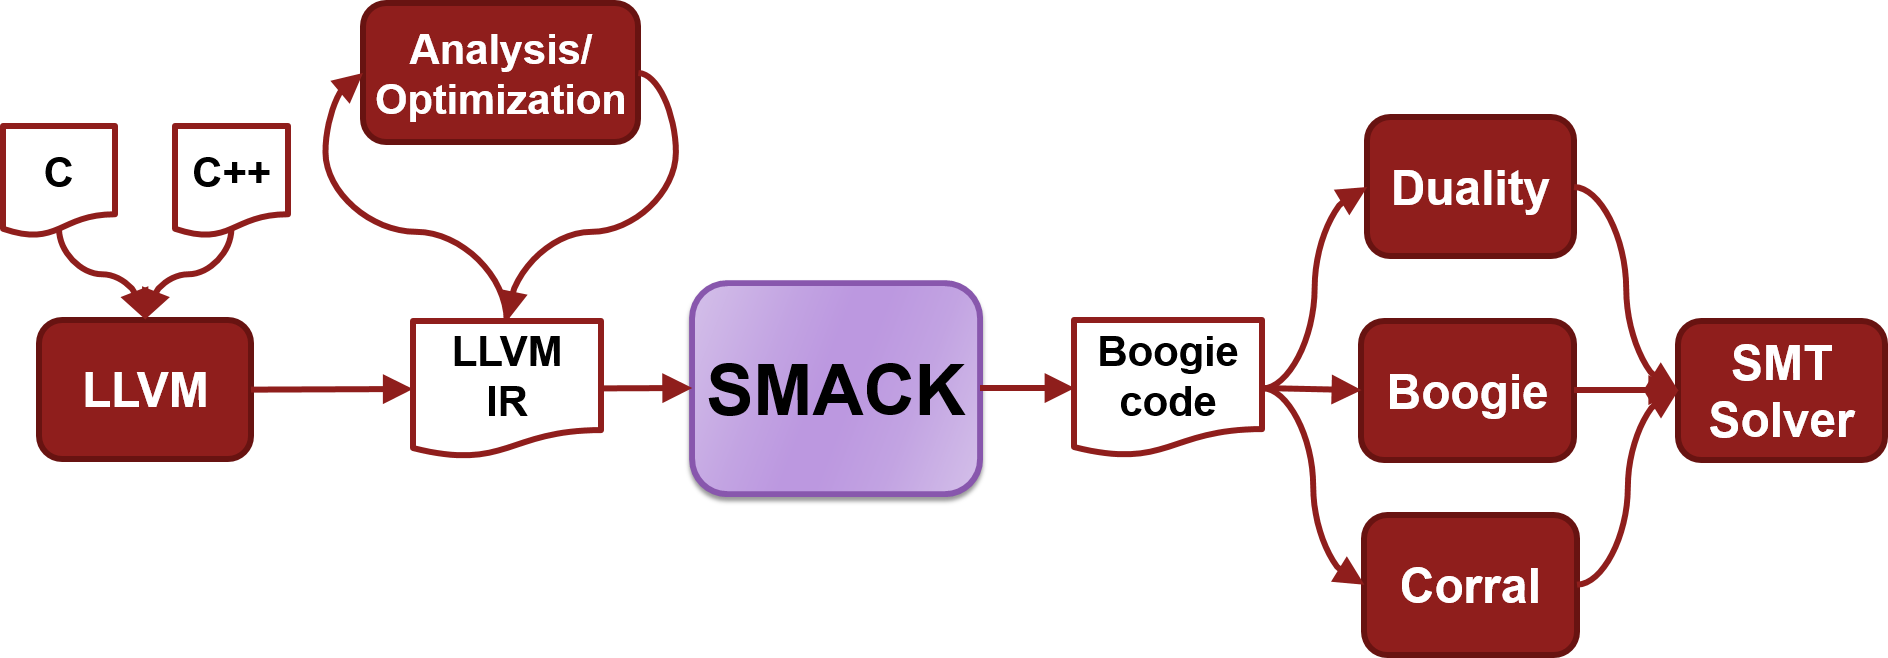
\includegraphics[width=1\textwidth]{SmackToolchain.png} 
  \caption{SMACK Toolchain}
  \label{fig:SMACKToolchain}
\end{figure}

The SMACK toolchain is depicted in Figure~\ref{fig:SMACKToolchain}.
Input C/C++ programs are given to Clang to compile and link, resulting
in an LLVM bytecode output.  This is then passed to the SMACK
executable, which translates the LLVM bytecode into a Boogie program
that models the behavior of the input C/C++ program.  The resulting
Boogie program is then passed to the back-end solver.  The solver
converts the Boogie program into an SMT query, which is then given to
one of the SMT solvers supported by the back-end solver for
evaluation. 

\section{Modeling Environment}\label{sec:modelingenvironment}
As described in Section~\ref{sec:smacktoolchain}, SMACK consumes LLVM
IR bytecode, builds a model of the input program, and generates a
Boogie IVL model of the input program.  The design of this toolchain
provides several levels at which modeling semantics can be
introduced. At the C level, external library functions that are
otherwise undefined can be given a definition, rather than verifying
the entire original source library. At the SMACK translation level,
undefined functions can be intercepted so SMACK can perform predefined
alterations to the translated Boogie program, rather than being
directly translated from the LLVM IR representation.  At the
translated Boogie level, additional variables and instructions can be
added to model environmental functionality that is not defined at the
C level. Finally, additional functionality can be modeled by the
back-end solver itself. 

To provide some context for the discussion of the modeling process,
the remainder of this chapter briefly introduces Boogie IVL, and then
discusses the mechanisms used for modeling, such as the Corral
concurrency primitives and C level Boogie injection.

\subsection{Boogie IVL}
The most illustrative way to introduce Boogie IVL is to simply show an
input C program and the relevant portions of the Boogie output that
SMACK returns. 
\begin{figure}[!ht]
\centering
\begin{subfigure}[b]{.45\textwidth}
\centering
\begin{lstlisting}


void main() {
  int *x, *y;
  x = malloc(sizeof(int));
  y = malloc(sizeof(int));
  *x = 1;
  *y = 2;
  assert(*x == 1);
}
\end{lstlisting}
\caption{Input C Code}\label{fig:cToBoogie_a}
\end{subfigure}
~
\begin{subfigure}[b]{.45\textwidth}
\centering
\begin{lstlisting}[language=boogie]
var $M: [int]int;

procedure main() {
  var $x, $y: int;
  call $x := $malloc(4);
  call $y := $malloc(4);
  $M[$x] := 1;
  $M[$y] := 2;
  assert($M[$x] == 1);
}
\end{lstlisting}
\caption{Boogie Code from SMACK}\label{fig:cToBoogie_b}
\end{subfigure}
\caption{SMACK Translation of C Program}\label{fig:cToBoogie}
\end{figure}

Figure~\ref{fig:cToBoogie_b} shows a reduced version of the Boogie
code as translated by SMACK from the input source depicted in
Figure~\ref{fig:cToBoogie_a}.  This simple program allocates space for
\lstinline|x| and \lstinline|y| on the heap, assigns values to each,
and then \lstinline|assert|s that the value of \lstinline|x| is as it
was assigned.  The Boogie translation reflects this, allocating space
on a model of the heap, \lstinline|$M|, and then indexing into this
array when storing and loading dynamic memory values.

\subsection{Corral Concurrency Primitives}
Corral is a state of the art solver for Boogie IVL programs.  One of
Corral's recent development efforts has been to improve support for
verifying concurrent programs.  To this end, Corral has extended
Boogie IVL, and recognizes the following concurrency primitives:

\begin{itemize}
\item \lstinline|async call|
  \emph{func}\lstinline|(|\emph{...}\lstinline|)| -- Asynchronously
  calls \emph{func} with the parameter list \emph{'...'} 
\item \lstinline|corral_atomic_begin()| -- Begins an atomic block
\item \lstinline|corral_atomic_end()| -- Ends an atomic block
\item \lstinline|corral_getThreadID()| -- Returns the ID of the
  calling thread.
\item \lstinline|corral_getChildThreadID()| -- Returns the ID of the
  most recently spawned thread
\end{itemize}

\begin{figure}[!ht]
\centering
\begin{lstlisting}[language=boogie]
var $x: int;
procedure f() modifies $x; {
  var $tid, $tmp: int;
  call $tid := corral_getThreadID();
  call corral_atomic_begin();
  $x := $tid;
  $tmp := $x
  call corral_atomic_end();
  assert($tmp == $tid);
}
procedure main() {
  var $ch1, $ch2: int;
  $x := 0;
  async call f();
  $ch1 := corral_getChildThreadID();
  async call f();
  $ch2 := corral_getChildThreadID();
  assert($x == $ch1 || $x == $ch2);
}
\end{lstlisting}
\caption{Utilizing Corral Concurrency Primitives}
\label{fig:corralprimitives}
\end{figure}


Figure~\ref{fig:corralprimitives} demonstrates the usage of each of
these primitives within the context of a complete Boogie program.
This program initializes the global variable \lstinline|$x| as 0, then
makes two asynchronous calls to the function \lstinline|f()| and
records the thread ID of each of the spawned threads of execution.  In
\lstinline|f()|, each of the spawned threads records their thread IDs.
Each thread then starts an atomic block, where it stores its thread ID
to the global \lstinline|$x| and then loads global \lstinline|$x| into
the local variable \lstinline|$tmp|.  The \lstinline|assert()| in
\lstinline|f()| should always succeed, since \lstinline|$x| is stored
and loaded within an atomic block. 

However, this program contains a bug.  Because there is no barrier
forcing the parent to wait for the child threads to execute, it is
possible that \lstinline|$x| will not be set to the thread ID of
either children by the time \lstinline|assert()| is called in
\lstinline|main()|.

\subsection{C Level Modeling}\label{sec:clevelmodeling}
Because there are several layers at which model semantics can be
introduced, SMACK has introduced several special C level functions
which insert model semantics at these various layers.
These special C level functions are not directly translated into
Boogie code, but, instead, are processed specially by SMACK.  This
allows users to introduce program semantics at the lower levels of the
modeling environment by writing code at the C level.  As a result, OS
environment and library models can be completely written as libraries
which get included C by input programs.  This avoids modifying SMACK's
source code directly in order to implement such models.

There are several C level functions that SMACK treats specially when
seen in the LLVM IR AST.  Upon seeing these, SMACK performs special
transformations to the Boogie translation, rather than translating the
function calls as they are.  Two of these functions were particularly
important for modeling the pthread extension to SMACK.

\begin{itemize}
\item \lstinline|__SMACK_code(char* format, ...)| -- Injects the
  string \lstinline|format| in the Boogie code.
\item \lstinline|__SMACK_top_decl(char* format, ...)| -- Inserts the
  string \lstinline|format| as a global declaration 
\end{itemize}

\begin{figure}[!ht]
\centering
\begin{subfigure}[b]{1\textwidth}
\centering
\begin{lstlisting}
void main() {
  __SMACK_top_decl("var $globalVar: int;");
  int *x;
  x = malloc(sizeof(int));
  *x = 1;
  __SMACK_code("$globalVar := @", *x);
  __SMACK_code("@ := $globalVar + 1", *x);
  assert(*x == 2);
}
\end{lstlisting}
\caption{Boogie Injecting C Code}\label{fig:cinjToBoogie_a}
\end{subfigure}
~
\begin{subfigure}[b]{1\textwidth}
\centering
\begin{lstlisting}[language=boogie]
var $globalVar: int;
var $M: [int]int;

procedure main() {
  var $x: int;
  call $x := $malloc(4);
  $M[$x] := 1;
  $globalVar := $M[$x];
  $M[$x] := $globalVar + 1;
  assert($M[$x] == 2);
}
\end{lstlisting}
\caption{Injected Boogie Translation}\label{fig:cinjToBoogie_b}
\end{subfigure}
\caption{Injecting Boogie Code from C}\label{fig:cinjToBoogie}
\end{figure}

Input to both of these functions is similar to that of C's
\lstinline|printf()| function; ``@'' symbols in the
\lstinline|format| string are replaced by arguments from the list
``...''.  Figure~\ref{fig:cinjToBoogie} demonstrates the C level usage,
and Boogie level translations of both of these functions.

The new implementation of pthread support for SMACK performs modeling
exclusively at the C code level, using these Boogie injection 
functions to model environmental state where necessary.

%%% Local Variables: 
%%% mode: LaTeX
%%% TeX-master: "thesis"
%%% End: 

\chapter{Model Design}\label{ch:modeldesign}
In this chapter, I discuss my research efforts toward developing a
model of the pthread library in SMACK.  I begin by introducing the
challenge of modeling the execution environment presented by the
operating system to the pthread library.  Having introduced this, I
proceed to discuss the process of modeling concurrency in the pthread
library over the lifecycle of a pthread.

\section{Execution Environment}
One of the critical tasks in implementing support for pthreads in
SMACK was modeling the environment that the operating system provides.
For each thread, the OS tracks the thread ID and thread status of
each thread spawned within a process.  This information is tracked by
the operating system in a thread control block (TCB).  At any time, a
thread must be able to query for its thread ID.  Similarly, a 
parent thread must be able to query the operating system for the
running state threads it has spawned.

Faithfully modeling the environment seen by the pthread library
requires addressing a number of bookkeeping issues.  These include
tracking the running state of each thread, and coordinating the thread
ID between the C level code and Corral itself.  The critical issue can
be illustrated by considering the API call
\lstinline|pthread_join(pthread_t* thr)|. This call blocks the calling
thread until the thread specified by \lstinline|thr| is in the stopped
state.  Consequently, properly model this function requires that the
calling thread must be able to query the environment for the status of
the thread referenced by \lstinline|thr|, in order to allow the
calling thread to unblock execution. 

Within the context of static model checking, because no code is
actually executing, the running state of a thread is simply a bit of
program state information -- a thread can be marked as waiting,
running, or stopped. Thus, tracking thread states requires the ability
to reference some bit of state information about the threads. A
\lstinline|pthread_t| object passed into \lstinline|pthread_join()|,
for example, must have some method of referencing this bit of thread
state information.  It seems natural to store each thread's thread ID
in this \lstinline|pthread_t| object, and use this to look up the
thread's state in an array.  Indeed, this is precisely how the
operating system tracks such information.  In addition, such an array
must be globally accessible, because threads must be able to query the
state of another thread (to singal \lstinline|pthread_join()|, for
example).  To model this, C level code is used to inject a global
Boogie-level array called \lstinline|$pthreadStatus|; the C level call

\begin{lstlisting}[frame=none,xleftmargin=2\parindent]
__SMACK_top_decl("var $pthreadStatus: [int][int]int;");
\end{lstlisting}

\noindent becomes

\begin{lstlisting}[frame=none,xleftmargin=2\parindent,language=boogie]
var $pthreadStatus: [int][int]int;
\end{lstlisting}

\noindent in the output Boogie program.

In order to access thread state from \lstinline|$pthreadStatus|, a
queried thread's thread ID is used to index into the array.  This
requires that a thread's ID is referenced by its
\lstinline|pthread_t| object.  This requires immediately querying
Corral for the thread ID of newly spawned thread, and recording this
information in its \lstinline|pthread_t|.  This is done from the
parent with \lstinline|corral_GetChildThreadID()|, and from the child
with \lstinline|corral_GetThreadID()|.  Now, when
\lstinline|pthread_join()|, for example, queries Corral for the
running state of a thread, it can pass in the thread ID to Corral,
which will use it to index into \lstinline|$pthreadStatus|.

However, there is further complication with implementing this
array. In Boogie, undefined variables take on a nondeterministic value
- that is, Corral assumes they can have any value.  Without
initializing \lstinline|$pthreadStatus|, Corral must consider the case
that threads start in a \emph{stopped} state.  This means that a call
to \lstinline|pthread_join()| immediately following a call to
\lstinline|pthread_create()| could query for the status of the newly
spawned thread before the new thread has initially set its status to
waiting, and see it is in the stopped state, causing the parent thread
to unblock.  To address this, \lstinline|$pthreadStatus| is
initialized so that all indices indicate an \emph{uninitialized}
state; the C level call 

\begin{lstlisting}[frame=none,xleftmargin=2\parindent]
__SMACK_code("assume (forall i:int :: "
                             "$pthreadStatus[i][0] == "
                             "$pthread_uninitialized);"); 
\end{lstlisting}

\noindent becomes 

\begin{lstlisting}[frame=none,xleftmargin=2\parindent,language=boogie]
assume (forall i:int :: $pthreadStatus[i][0] == 
                        $pthread_uninitialized);
\end{lstlisting}

\noindent in the output Boogie program.  This code gets executed as
the first statement in \lstinline|main()|, to ensure that any thread's
running state is defined prior to its use. 

With these Boogie level additions to each pthread program's Boogie
translation, the operating system environment is sufficiently prepared
to enable the modeling of the actual pthread library behavior.


\section{Thread Creation}
With the pthread library's execution environment modeled, a sufficient
framework exists to begin modeling the behavior of the actual pthread
library function calls.  In the pthread library, the procedure for
spawning threads is \lstinline|pthread_create()|.  There are two
aspects of \lstinline|pthread_create()| that require modeling:
behavior in the calling thread, and behavior in the newly spawned
thread. 

In the calling thread, there are two main tasks.  As the first task,
the new thread must be spawned, and instructed to execute the
procedure indicated by the \lstinline|*__start_routine| function
pointer.  As the second, SMACK must query Corral for the thread ID of
the newly spawned child thread, and record this value in the
\lstinline|pthread_t| struct for future reference.  This results in
the model defined in the C code seen in Figure~\ref{fig:pthread_create}.

\begin{figure}[h]
\centering
\caption{Model: pthread\_create()}\label{fig:pthread_create}
\begin{lstlisting}
int pthread_create(pthread_t* __newthread,
                   pthread_attr_t* __attr,
                   void* (*__start_routine) (void *),
                   void* __arg)
{
  __SMACK_code("async call @(@, @, @);", __call_wrapper,
                                         __newthread,
                                         __start_routine,
                                         __arg);

  __SMACK_code("call @ := corral_getChildThreadID();",
               *__newthread);

  return 0;
}
\end{lstlisting}
\end{figure}

In the newly spawned thread, again there is bookkeeping to do, as well
as executing the specified \lstinline|__start_routine()|.  Notice in
Figure~\ref{fig:pthread_create} that the function
\lstinline|__call_wrapper()| is the procedure being executed
asynchronously, rather than \lstinline|__start_routine()|.  This
allows for the child thread to perform bookkeeping before and after
calling \lstinline|__start_routine()|.

As seen in Figure~\ref{fig:__call_wrapper} the newly spawned thread
queries Corral for its thread ID, and then makes a call to
\lstinline|assume()|, which causes Corral to only consider paths
through the program where \lstinline|*__newthread| already contains
the thread ID of the child thread -- effectively, the new thread
``waits'' until its parent has set the child thread's ID in
\lstinline|*__newthread|. Once this has occurred, both the parent and
the child have a reference to the newly spawned thread's ID, and can
use this to index into \lstinline|$pthreadStatus| to set and query the
child thread's running state information.  

Once the child and parent can both reference the correct
\lstinline|$pthreadStatus| element, the new thread can proceed to
executing the specified \lstinline|__start_routine()|.  The new thread
cycles through the \emph{waiting} state to the \emph{running} state,
and then makes a synchronous call to the
\lstinline|__start_routine()|.  After the
\lstinline|__start_routine()| returns, the thread's running state is
finally set to \emph{stopped}, which signals the end of the child
thread. 

\begin{figure}[h]
\centering
\caption{Model: \_\_call\_wrapper()}\label{fig:__call_wrapper}
\begin{lstlisting}
void __call_wrapper(pthread_t* __newthread,
                    void* (*__start_routine)(void *),
                    void* __arg)
{
  int ctid = __SMACK_nondet();
  __SMACK_code("call @ := corral_getThreadID();", ctid);
  assume(ctid == *__newthread);
  
  __SMACK_code("$pthreadStatus[@][0] := $pthread_waiting;",
               *__newthread);
  __SMACK_code("$pthreadStatus[@][0] := $pthread_running;",
               *__newthread);

  __start_routine(__arg);

  __SMACK_code("$pthreadStatus[@][0] := $pthread_stopped;",
               *__newthread);
}
\end{lstlisting}
\end{figure}



\section{Thread Execution}
[Good]
With the ability to spawn threads, [wc it becomes time to] consider
the functionality of the pthread library that pertains to an executing
thread.  Among this functionality, the most commonly utilized are the
synchronization routines.

Corral extends Boogie IVL with two primitives for achieving
synchronization between threads: \lstinline|corral_atomic_begin()| and
\lstinline|corral_atomic_end()|.  These calls provide the ability to
create critical sections of Boogie IVL code, where only one atomic
block can execute at any time.  However, these atomic blocks are
global, and take no parameters.  There is no way to differentiate
atomic blocks of unrelated code that should be allowed to run
concurrently -- this is much like the big kernel lock in Linux.  This
presents the need to model the more complex synchronization routines
of pthreads using Corral's atomic primitives.

\subsection{Modeling Mutexes}
[Good]
Mutexes are the most commonly used mechanisms for providing
synchronization among threads.  In addition, they can be used as
building blocks to devise more complex synchronization mechanisms.
Modeling mutexes in Corral is relatively straightforward, and more
complex synchronization functionality easily builds on this
foundation. 

Each \lstinline|pthread_mutex_t| object allocated creates an
independent mutual exclusion device.  To track the current owner of a
mutex and prevent execution of threads that don't hold the lock, the
model stores the thread ID of the current mutex owner in the
\lstinline|pthread_mutex_t| struct.  This allows
\lstinline|pthread_mutex_lock()| to block until until the mutex is in
the \emph{UNLOCKED} state.


\begin{figure}[h]
\centering
\caption{Model: pthread\_mutex\_lock()}\label{fig:pthread_mutex_lock}
\begin{lstlisting}
int pthread_mutex_lock(pthread_mutex_t* __mutex)
{
  int tid = (int)pthread_self();
  assert(__mutex->init == INITIALIZED);
  assert(__mutex->lock != tid);

  __SMACK_code("call corral_atomic_begin();");
  assume(__mutex->lock == UNLOCKED);
  __mutex->lock = tid;
  __SMACK_code("call corral_atomic_end();");

  return 0;
}
\end{lstlisting}
\end{figure}

This leads to the straightforward model shown in
Figure~\ref{fig:pthread_mutex_lock}. The calling thread queries for
its thread ID using \lstinline|pthread_self()| (which simply queries
Corral with a call to \lstinline|corral_GetThreadID()|, and returns the
result). The mutex is then checked to ensure it is in the initial
state, and that the calling thread is not already the owner of the
mutex.  With these criteria ensured, the Boogie translation atomically
waits for the mutex to enter the \emph{UNLOCKED} state and updates the
mutex owner to be the calling thread's ID.

\lstinline|pthread_mutex_unlock()|, seen in
Figure~\ref{fig:pthread_mutex_unlock}, releases a mutex, and is
essentially the inverse of \lstinline|pthread_mutex_lock()|; the model
ensures the mutex is initialized and the calling thread is the current
owner, and atomically sets the mutex as being unlocked. 

\begin{figure}[h]
\centering
\caption{Model: pthread\_mutex\_unlock()}
\label{fig:pthread_mutex_unlock}
\begin{lstlisting}
int pthread_mutex_unlock(pthread_mutex_t* __mutex)
{
  int tid = (int)pthread_self();
  assert(__mutex->init == INITIALIZED);
  assert(__mutex->lock == tid);

  __SMACK_code("call corral_atomic_begin();");
  __mutex->lock = UNLOCKED;
  __SMACK_code("call corral_atomic_end();");

  return 0;
}
\end{lstlisting}
\end{figure}

\subsection{Complex Synchronization}
[Short, but sufficient?]
The pthread library also includes a number of more complex
synchronization mechanisms.  These allow for more efficient runtime
behavior, in addition to providing commonly utilized synchronization
mechanisms.

\lstinline|pthread_cond_wait(pthread_cond_t* cond, |
\lstinline|pthread_mutex_t* mutex)|  is one such function that
provides more efficient runtime behavior.  It blocks the calling
thread until both the \lstinline|cond| predicate is true \emph{and}
\lstinline|mutex| is \emph{UNLOCKED}, at which point the thread is
signaled to resume. This avoids having to continually acquire the
mutex and evaluate the predicate.  \lstinline|pthread_barrier_wait()|
is a good example of a procedure providing expected functionality.  It
causes calling threads to block until all threads calling
\lstinline|pthread_barrier_wait()| have reached this instruction.
These more complex synchronization routines are modeled entirely as C
level code simply by using \lstinline|pthread_mutex_t|'s as building
blocks. 

\section{Thread Termination}
[Good]
As a thread's execution comes to an end, there is a bit of bookkeeping
to be done to wrap up the thread's lifecycle.  It is primarily this
termination handling that required the upfront work of modeling the
operating system environment prior to implementing support for thread
creation.

There are two main considerations for handling the termination of a
thread.  The first consideration is the passing of a return value from
a terminating thread.  The second is blocking execution of a waiting
thread, and retrieving the return value of the terminating thread
being waited on by the blocking thread.

\subsection{Modeling Thread Exit and Join}
[Could use another pass or two]
It is often necessary to pass a return value from a terminating thread
to some other thread.  For example, with a scatter/gather design
pattern, a parent thread will send data to multiple worker threads,
which return a computational result back to the parent.

The challenge with achieving this was that this return data has to
exist somewhere between the time that the terminating thread exits,
and the joining thread retrieves it.  This functionality was
implemented by extending the definition of the
\lstinline|$pthreadStatus| array to store a tuple, rather than a 
single value.  With this, the model can store a return value passed
into \lstinline|pthread_exit(void* value)| as the second tuple
element, in addition to storing thread running state as the first.

\begin{figure}[h]
\centering
\caption{Model: pthread\_exit()}\label{fig:pthread_exit}
\begin{lstlisting}
void pthread_exit(void *retval)
{
  pthread_t tid = __SMACK_nondet();
  tid = pthread_self();

  __SMACK_code("assert $pthreadStatus[@][0] == "
               "$pthread_running;",
               tid);

  __SMACK_code("$pthreadStatus[@][1] := @;", tid, retval);

  __SMACK_code("$pthreadStatus[@][0] := $pthread_stopped;",
               tid);
}
\end{lstlisting}
\end{figure}

The model of \lstinline|pthread_exit()|, seen in
Figure~\ref{fig:pthread_exit}, gets the calling thread's ID and
ensures the thread is still in a running state, saves the return value
pointer in \lstinline|$pthreadStatus|, and finally sets the running to
stopped.  


With the return value from threads now stored in
\lstinline|$pthreadStatus|, a method for accessing this value is
needed.  This is done through 
\lstinline|pthread_join(pthread_t* thr)|, which blocks the calling
thread until the thread referenced  by \lstinline|thr| terminates.
The value returned from \lstinline|pthread_join()| is the pointer
passed in to \lstinline|pthread_exit()| by the terminating thread.

The model designed for \lstinline|pthread_join()|, shown in
Figure~\ref{fig:pthread_join} implements this behavior.  A call to
\lstinline|assume()| causes the thread to block until the target
thread's running state is \emph{stopped}.  Once the terminating thread
is stopped, the waiting thread fetches the return value pointer from
the \lstinline|$pthreadStatus| array, which is then returned by the
call to \lstinline|pthread_join()|.

\begin{figure}[h]
\centering
\caption{Model: pthread\_join()}\label{fig:pthread_join}
\begin{lstlisting}
int pthread_join(pthread_t __th, void **__thread_return)
{
  __SMACK_code("assume $pthreadStatus[@][0] == "
               "$pthread_stopped;",
               __th);

  __SMACK_code("@ := $pthreadStatus[@][1];",
               *__thread_return, __th);

  return 0;
}

\end{lstlisting}
\end{figure}

%%% Local Variables: 
%%% mode: latex
%%% TeX-master: "thesis"
%%% End: 

\chapter{Implementation}\label{ch:implementation}
With the model of the pthread library in place, the next step in my
research was to look forward and consider the actual implementation of
phtread library support as part of the SMACK verifier.  This chapter
provides an overview of the actual implementation of pthread library
support within SMACK.  I begin the chapter with a specification of the
goals targeted for the pthread extension to SMACK.  Next, I describe
the mechanism used for including the model within SMACK.  \iffalse
[This is followed by a discussion of changes required in the SMACK
tool itself to support the new model.]\fi  I conclude the chapter with
a description of the current state of the implementation in relation
to the implementation goals. 

\section{Implementation Goals}\label{sec:implementationgoals}
There were two main motivations encouraging the implementation of
support for programs utilizing pthreads within SMACK.  The first, as
mentioned in Chapter~\ref{ch:introduction}, were requests from the
SMACK user community.  The second was to improve SMACK's performance
in the SVCOMP software verification competition.  SVCOMP is an
international software verification, and is co-located with the TACAS
conference, competition.  Last year SMACK made its debut appearance at
SVCOMP, but had several categories in which it was unable to compete;
pthreads was one of these categories.

The specific needs of these two motivators largely overlap; both
require support for the most commonly utilized functionality of the
pthread library.  To assess the most commonly utilized functionality,
I collected benchmarks from SVCOMP, as well as from the Inspect and
CIVL projects to diversify the sample of benchmarks.  This collection
was then scanned for calls into the pthread API.  A count of the
number of occurrences for each call was generated, and the pthread API
procedures prioritized for modeling according to their frequency of
occurrence within this sample set. 

This analysis yielded some good insight into the commonly utilized
functionality of the pthread library.  As expected, the basic
procedures such as \lstinline[breaklines]|pthread_create()|,
\lstinline[breaklines]|pthread_join()|,
\lstinline[breaklines]|pthread_mutex_lock()| and 
\lstinline[breaklines]|pthread_mutex_unlock()| were at the top of the
list. However, functionality such as error handling options as well as
attribute setters/getters controlling the behavior of things such as
multiprocess mutex scope and thread scheduling had very few calls, if
any.  As a result, these type of features were left as future
work. The final set of modeled API calls can be seen in
Section~\ref{sec:implementationstatus}.  

\section{Model Inclusion}
As mentioned in Section~\ref{sec:modelingenvironment}, libraries
included by input programs are not typically linked when SMACK
generates LLVM bytecode.  The functions declared in these library
headers go undefined, and SMACK models their behavior as returning a
nondeterministic value, though not affecting program state.  In this
regard the pthread library was no different.  SMACK would treat a call
to \lstinline|pthread_create()| as simply returning a nondeterministic
integer, with no threads spawned or functions called. 

Generally, the strategy for adding a model to SMACK is as simple as
providing a definition for the functions declared in library headers.
Once a definition has been provided for a function included in a
library header, SMACK will find the function definition and translate
the function definition with the rest of the input program.  As a
result, a call to such a function will use the modeled behavior,
rather than returning a nondeterministic value.

Because SMACK uses Clang to compile input programs to LLVM bytecode,
these externally defined functions can be referenced by the input
C/C++ program the same way that externally defined functionality is
added to any C/C++ program. Header files are included to declare the
functions, and calls to the functions are resolved by the linker to
point the definitions contained in the compiled library file.

This strategy of providing a replacement library containing a model
of the original library is precisely how the pthread model discussed
in Chapter~\ref{ch:modeldesign} was added to SMACK.  When SMACK calls
Clang, it passes the \emph{-I} switch with the path to the replacement
\lstinline[identifierstyle=\color{black}]|pthread.h|.  This causes the
SMACK version of \lstinline[identifierstyle=\color{black}]|pthread.h|
to be included, rather than searching the default include paths and
using the system \lstinline[identifierstyle=\color{black}]|pthread.h|.
With our declarations of the pthread API included, the compiled input
program bytecode is then linked with the bytecode compiled from the C
source file containing our model of the pthread library. As a result,
the AST seen by SMACK during translation to Boogie contains the
pthread library models described in Chapter~\ref{ch:modeldesign}.

\iffalse
\section{SMACK Modification?}
[Maybe delete this section, depending on time]
[Do a section here on init funcs?]

In addition to linking the pthread model during compilation of LLVM IR
bytecode, there were[are?] two additional problems related to LLVM IR
to Boogie translation [how to say smack itself?] that needed to be
addressed.

The first problem is related to the initialization of the
\lstinline|$pthreadStatus| array, which sets all threads to an
\emph{uninitialized} state, as described in
Section~\ref{sec:executionenvironment}.  This initialization must
be performed from a within a call to a function, as neither C/C++ nor
Boogie allow statements to be executed in the global declaration
scope.  To ensure this initialization happens before any code other
input program code is evaluated, this initialization of
\lstinline|$pthreadStatus| must be injected as the first statement in
\lstinline|main()|.  This required extending SMACK itself with an
additional C level Boogie injection function, similar to those
described in Section~\ref{sec:clevelmodeling}.  The added functionality
causes SMACK to search for function definitions whose function name
starts with \lstinline|__SMACK_init_func_|.  Any such function
definition encountered while parsing the AST causes SMACK to insert a
call to the function as the first line of \lstinline|main()|.  This
allows such functions to be defined in modeled libraries, rather than
having to modify the source of each input program requiring such an
initialization.  It is using this new functionality that
\lstinline|$pthreadStatus| is initialized. 

The second problem is the ability of a function call to inform SMACK
that the thread of execution is stopping, such as with the
\lstinline|exit()| system call, or \lstinline|pthread_exit()|.  As
with modeling the operating system environment's thread ID coordination,
terminating a thread of execution is similarly the operating system's
responsibility.  When the operating system receives the
\lstinline|exit()| system call, it proceeds to swap out the process,
and mark it as \emph{stopped}.  There is no Boogie IVL instruction for
this, so it must be modeled.  There are several proposals for
addressing this, but it currently remains unimplemented.
\fi

\section{Implementation Status}
\label{sec:implementationstatus}
Currently, there are 15 pthread API calls modeled in the pthread
extension to SMACK.  These 15 calls represent 2959 of 3257 of all
pthread API calls found in the SVCOMP, Inspect, and CIVL
benchmarks. At roughly 91\%, this covers a significant majority of the
calls into the pthread API library found in the benchmark programs.
Further, some of the missing 300 were explained with a quick check
through the benchmarks which revealed calls to functions like
``\lstinline|my_pthread_mutex_lock()|''.  Despite this, there remain
several pthread API functions unimplemented, such as those alluded to
in Section~\ref{sec:implementationgoals}. 


In its present form, the pthread extension to SMACK models the
following pthread API calls:

\begin{multicols}{2}
\begin{itemize}
\item \lstinline|pthread_create()|
\item \lstinline|pthread_self()|
\item \lstinline|pthread_exit()|
\item \lstinline|pthread_join()|
\item \lstinline|pthread_mutex_init()|
\item \lstinline|pthread_mutexattr_init()|
\item \lstinline|pthread_mutexattr_settype()|
\item \lstinline|pthread_mutex_lock()|
\item \lstinline|pthread_mutex_unlock()|
\item \lstinline|pthread_mutex_destroy()|
\item \lstinline|pthread_cond_init()|
\item \lstinline|pthread_cond_wait()|
\item \lstinline|pthread_cond_signal()|
\item \lstinline|pthread_cond_broadcast()|
\item \lstinline|pthread_cond_destroy()|
\end{itemize}
\end{multicols}

With the most commonly used pthread functions modeled, the pthread
extension to SMACK is certainly ready for experimental use, and even
real-world use with programs that don't fully utilize the pthread
API. 

%%% Local Variables: 
%%% mode: latex
%%% TeX-master: "thesis"
%%% End: 

\chapter{Empirical Evaluation}\label{ch:evaluation}
In order to assess the accuracy and performance of the newly
implemented pthread extension to SMACK, regression testing and
benchmarking was performed to exercise the new model.  The design and
results of these tests are described in this section. 

\section{Methodology}
[Describe experimental setup.]

\section{Results \& Analysis}
[Deliver the goods]

\begin{table}[h]
\centering
\caption{SVCOMP Benchmark Results}\label{table:benchmarkresults}
\begin{tabular}{|l|l|l|l|l|l|}
\hline 
Benchmark                  & LOC & \# Thrd & Ctx Switches & SMACK RT        & Lazy-CSeq RT   \\
\hline\hline
dekker\_true.c             & 62  & 3       & 3            & 2 s             & 4 s            \\
\hline
lamport\_true.c            & 83  & 3       & 3            & 3 s             & 5 s            \\
\hline
lazy01\_false.c            & 57  & 4       & 2            & 5 s             & 1 s            \\
\hline
peterson\_true.c           & 49  & 3       & 3            & 2 s             & 2 s            \\
\hline
qrcu\_false.c              & 155 & 4       & 3            & 102 s           & 1 s            \\
\hline
queue\_false.c             & 185 & 3       & 2            & 180 s (SIZE=10) & 18 s (SIZE=20) \\
\hline
queue\_ok\_true.c          & 160 & 3       & 2            & 295 s (SIZE=10) & 51 s (SIZE=20) \\
\hline
reorder\_2\_false.c        & 90  & 5       & 2            & 4 s             & 2 s            \\
\hline
reorder\_5\_false.c        & 88  & 6       & 2            & 11 s            & 3 s            \\
\hline
sigma\_false.c             & 55  & 6       & 2            & 85 s            & 9 s            \\
\hline
singleton\_false.c         & 64  & 7       & 2            & 75 s            & 3 s            \\
\hline
stack\_false.c             & 127 & 3       & 2            & 18 s            & 1 s            \\
\hline
stack\_true.c              & 131 & 3       & 2            & 731 s           & 77 s           \\
\hline
stateful01\_false.c        & 62  & 3       & 2            & 5 s             & 1 s            \\
\hline
stateful01\_true.c         & 62  & 3       & 2            & 14 s            & 3 s            \\
\hline
sync01\_true.c             & 71  & 3       & 2            & 27 s            & 3 s            \\
\hline
szymanski\_true.c          & 62  & 3       & 2            & 2 s             & 3 s            \\
\hline
time\_var\_mutex\_true.c   & 62  & 3       & 2            & 22 s            & 3 s            \\
\hline
twostage\_3\_false.c       & 136 & 4       & 2            & 19 s            & 2 s            \\
\hline
qrcu\_true.c               & 155 & 4       & 3            & N/A             & 52 s           \\
\hline
read\_write\_lock\_false.c & 59  & 5       & 2            & N/A             & 1 s            \\
\hline
read\_write\_lock\_true.c  & 57  & 5       & 2            & N/A             & 6 s            \\
\hline
scull\_true.c              & 477 & 4       & 2            & N/A             & 5 s            \\
\hline
sssc12\_true.c             & 43  & *       & 2            & N/A             & 14 s           \\
\hline
\end{tabular}
\end{table}


%%% Local Variables: 
%%% mode: latex
%%% TeX-master: "thesis"
%%% End: 

\chapter{Conclusions \& Future Work}\label{ch:conclusion}
Initial results of benchmark testing prove to be very encouraging with
regard to the 







In conclusion, I concluded that this conclusion is too short and off
topic.








[left over from this chapter, but out of place here]
[This paragraph feels like it belongs somewhere else]
There are two main reasons for modeling a library instead of including
it as part of the input program.  The first reason is to abstract away
interaction with the operating system and hardware.  Directly
including the pthread library as part of input programs would require
a model of the OS system calls, kernel data, an environmental behavior
that the pthread library accesses.  The engineering cost of doing this
is greater than model the pthread library itself.  The second reason
is that modeling a library greatly reduces the computational
complexity of verification.  A brief glance at the pthread library
source reveals much longer, more complex code than the model designed
in Chapter~\ref{ch:modeldesign}.

[leftover from intro]
[Remaining is leftover stuff -- may be useful when revising intro]
This is supported by the accuracy seen in the empirical results of
initial implementation testing.  My proposed research will extend
SMACK with a model of a common subset of the pthreads API, enabling
verification of C/C++ programs utilizing the Pthreads library.
Extending SMACK to provide support for programs using pthreads has not
only provided the SMACK community with support for a common
concurrency paradigm, but also presents an opportunity to investigate
general constructs useful for modeling concurrency.  These constructs,
which will necessarily result from extending SMACK, will lend
themselves to modeling other concurrency libraries like OpenMP and
MPI.  Further, the resulting constructs should be general enough for
use within other verification tools. 



%%% Local Variables: 
%%% mode: latex
%%% TeX-master: "thesis"
%%% End: 


% end matter
\numberofappendices=0
%\appendix
%\include{appA}



%Set chapters back up a level for pdf bookmarks so references isn't in
%the "Chapters" header
\makeatletter
\renewcommand{\toclevel@chapter}{0}
\renewcommand{\toclevel@section}{1}
\renewcommand{\toclevel@subsection}{2}
\renewcommand{\toclevel@subsubsection}{3}
\renewcommand{\toclevel@paragraph}{4}
\renewcommand{\toclevel@subparagraph}{5}
\makeatother
\nocite{*}
\bibliographystyle{ieeetr}
\bibliography{thesis_bib}

\end{document}

%%% Local Variables:
%%% TeX-master: "thesis"
%%% End: